
\begin{abstract}

「递归自我改进」（RSI）在过去四年从一句愿景变成了一批可运行的系统：模型自己出题、自己解题、自己当裁判、自己改自己的代码，甚至自己改进「改进的方法」。本文对这 61 篇工作做系统梳理，要回答的不是「能不能做到」，而是\textbf{这些闭环究竟在改什么，支撑它们的证据有多强}。


梳理得到一个与直觉不同的判断：真正的变化不在算法，而在\textbf{判断权的位置}。按「改什么」可分五层——上下文、外壳、评判器、权重、改进过程——而层与层之间最关键的区别不是效果大小，是\textbf{单次改动能否被验证、失败能否被回滚}。这两个性质同向变化：越往下，越不可验证、越难回滚。


在这个分层下，四年演进的形状变得清楚：外部锚点沿「人写答案 \sym{→}{} 可判定答案 \sym{→}{} 模型判断 \sym{→}{} 统计量」单向内移。27 篇改权重的工作里，以可判定答案为奖励的 20 篇、以模型判断为奖励的 5 篇、以统计量替代判定的 3 篇。每内移一步都换来更大的可扩展性：从需要人工推理，到只需要一个测试，到只需要一个通过/不通过，最后到只需要一个标量。但每一步也都换来一类新的失效——判断者与被判断者同源，带来自我确认循环与判据饱和；用置信度代替对错，带来与目标的脱钩；改外壳带来验收门的失明，因为门只看得见分数，看不见自己正在拆掉第几层防护。


证据强度的落差比失效模式更值得警惕。对 90 篇自称 RSI 的研究，只有 22\% 审计了两次以上的完整循环。而唯一能回答「能力边界有没有移动」的指标 pass@k，在本文编码的 61 篇里只有 2 篇报告——被最少报告的指标，恰好是最难看的那个。


\textbf{关键词}：递归自我改进；自举；可验证奖励；自我确认循环；模型坍缩；评测审计


\end{abstract}
\section{引言}

\subsection{一个词，五种东西}

「自我改进」在文献里至少有五种互不兼容的用法。它可能指模型改自己的提示，也可能指改自己的代码，也可能指改自己的权重、自己的评判器，甚至自己改进的方法。


这个领域用同一套词汇（self-refine、self-reward、self-play、self-evolve）覆盖了根本不同的志向 {\scriptsize\texttt{[c-\hspace{0pt}rsi-\hspace{0pt}vocabulary]}}。后果是可比较性丧失——两篇都叫 self-improving 的论文，可能一篇的失败可以删一行记录撤销，另一篇的失败只能重训。


本文的第一个任务就是把这个词拆开。拆分需要一个操作性的判据：\textbf{RSI 与自改进的区别不在效果大小，而在闭环的闭合度——被改进的对象是否包含「改进机制本身」} {\scriptsize\texttt{[c-\hspace{0pt}rsi-\hspace{0pt}definition]}}。DGM 改的是「自己改代码的能力」，是这一判据的最小实例；STaR 改的是模型参数，而改进机制（人选的循环）没有被改。


\subsection{三个问题}

\begin{itemize}
  \item \textbf{Q1}：这些闭环在改什么？能否拆成可比较的层次？
  \item \textbf{Q2}：奖励信号从哪里来？它在往哪个方向移动？
  \item \textbf{Q3}：这些工作的证据，能不能支撑它们使用的词？
\end{itemize}

第三个问题最不讨喜，但它是本文的重点。前两个问题已有综述在回答，第三个问题的答案直到 2026 年才第一次被系统测量。


\subsection{贡献}

\begin{enumerate}
  \item 给出一个可操作的五层分层，并指出\textbf{可验证性与回滚成本同向}，据此可以直接推出「哪一层可以放开自动改」。
  \item 把奖励来源编码成可复算的分布，指出锚点内移不是比喻而是一个可统计的趋势，并说明每一步内移换来了什么、失去了什么。
  \item 把「证据强度」当作独立的研究对象：不问这些工作对不对，而问它们提供的证据能不能支撑它们使用的词。
\end{enumerate}

\section{方法：语料与编码}

\subsection{检索与纳入}

检索窗口 2022-01 至 2026-11，用 16 组 arXiv 检索式取并集，得到候选池 1006 篇。按「提出或测量一个自举闭环」纳入 61 篇（2022-03 至 2026-11），编码为三个维度：改什么（layer）、奖励从哪来（reward）、摘要报什么指标（metric）。全部编码写在 \texttt{corpus\_labels.csv}，统计由 \texttt{analyze.py} 重算。


纳入的 61 篇按年份分布为 2022 年 1 篇、2023 年 9 篇、2024 年 14 篇、2025 年 22 篇、2026 年 15 篇 {\scriptsize\texttt{[c-\hspace{0pt}corpus-\hspace{0pt}timeline]}}（图 1）。2026 年只统计到 11-05，这个数不应读作降温。


\begin{figure*}[t]
\centering
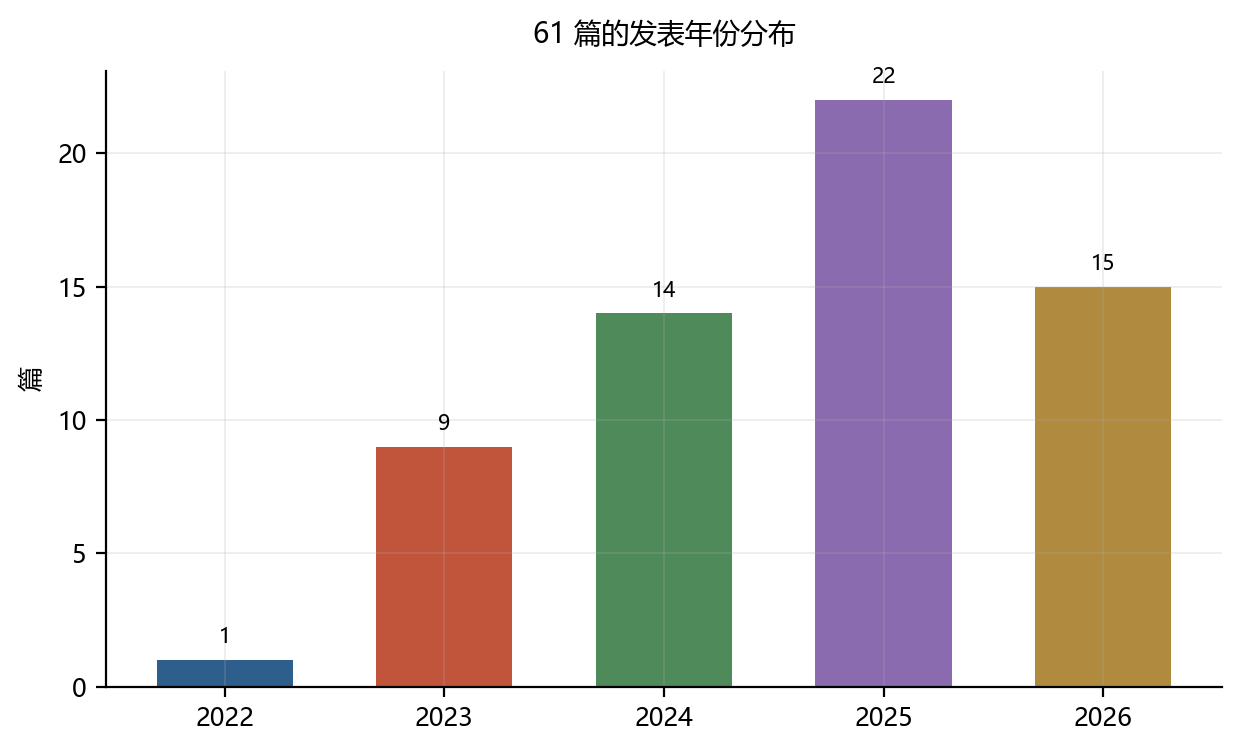
\includegraphics[width=0.86\textwidth]{../figures/fig-1.png}
\caption{图 1　61 篇按发表年份分布。2025 年是峰值（22 篇）；2026 年只统计到 11-05，不应读作降温。}
\label{fig:1}
\end{figure*}

一处必须声明的偏差：首轮凭记忆列出的 66 个经典工作 arXiv ID 里，有 11 个是错的——标题配到了别的论文上。全部经 \texttt{id\_list} 逐条核对后剔除，或改由标题检索补回。这件事的教训写在 §10.2：\textbf{校验器检查引用是否闭合，不检查引用是否指向你以为的那篇论文。}


\subsection{证据链的三级结构}

本文的每条判断都可回溯到三级：正文的方括号标记（形如 \texttt{[c-anchor-migration]}）指向一条\textbf{主张}，主张指向\textbf{证据}（arXiv 摘要的原文片段），证据指向\textbf{来源}（53 条 arXiv 预印本）。本文引用的 48 条主张、63 条证据，全部记录在归档的 CSV 里。


两条纪律值得单独说明。第一，所有 63 条引文都是从摘要中原样摘取的子串，写入前逐条校验，不做近似匹配。第二，凡涉及计数的数字（27 篇权重层、20 篇答案奖励等），都在主张里写明可重算的推导式，由审计脚本从语料重新数一遍——不是信任作者的数，而是逼它可复现。


\section{分层：改的到底是什么}

\subsection{五层}

按「改什么」分层是本档的操作性定义 {\scriptsize\texttt{[c-\hspace{0pt}loop-\hspace{0pt}layers]}}：


\begin{itemize}
  \item \textbf{上下文层}：反思记录、记忆、技能库。模型不动，状态动。
  \item \textbf{外壳层}：代码、提示、工作流。模型不动，外围的代码动。
  \item \textbf{评判器层}：judge、reward model、verifier。判断标准本身被改进。
  \item \textbf{权重层}：模型参数。
  \item \textbf{过程层}：改进机制本身——即「以后怎么改」这件事被改。
\end{itemize}

\begin{table*}[t]
\centering
\footnotesize
\setlength{\tabcolsep}{4pt}
\caption{五层分层与它的两个性质。分层是本文的构造；回滚成本与可验证性同向，这是第 8 节建议的依据。}
\label{tab:1}
\begin{tabularx}{\textwidth}{lXll}
\toprule
层 & 改的对象 & 回滚成本 & 单次改动的可验证性 \\
\midrule
上下文 & 反思、记忆、技能库 & 极低（删记录） & 高（同模型同任务可比） \\
外壳 & 代码、提示、工作流 & 低（回退版本） & 高但有陷阱（验收门会掩盖防护流失） \\
评判器 & judge / reward model / verifier & 中 & 中（评判器本身要被评判） \\
权重 & 模型参数 & 高（重训） & 低（一次更新无法归因） \\
过程 & 改进机制本身 & 最高 & 最低（改后此前验证全部失效） \\
\bottomrule
\end{tabularx}
\end{table*}

分层本身不是新东西——自演化 agent 的综述早就按「模型、记忆、工具、架构」分过。两篇综述给出的出发点也是同一个：模型本身是静态的，不会随任务改变内部参数；而推理时自改进把增益放在计算而不是参数上 {\scriptsize\texttt{[c-\hspace{0pt}survey-\hspace{0pt}framing]}}。这恰好解释了为什么「自我改进」能同时容纳两条互不兼容的路线。


本文这张表的用处不在分类，在\textbf{最后两列}：回滚成本与单次改动的可验证性。这两列同向。上下文层的改动可以删一条记录撤销，验收就是「同一模型在同一任务上是否更好」；权重层的改动要重训，而且一次更新无法归因到具体哪条数据。过程层最糟：改了改进机制之后，\textbf{此前所有的验证结论都要作废}，因为你验证的是旧的机制。


\subsection{分布}

61 篇的构成是：权重层 27 篇、外壳层 13 篇、分析类 15 篇、上下文层 4 篇、评判器层 1 篇、过程层 1 篇 {\scriptsize\texttt{[c-\hspace{0pt}corpus-\hspace{0pt}composition]}}（图 2）。


\begin{figure*}[t]
\centering
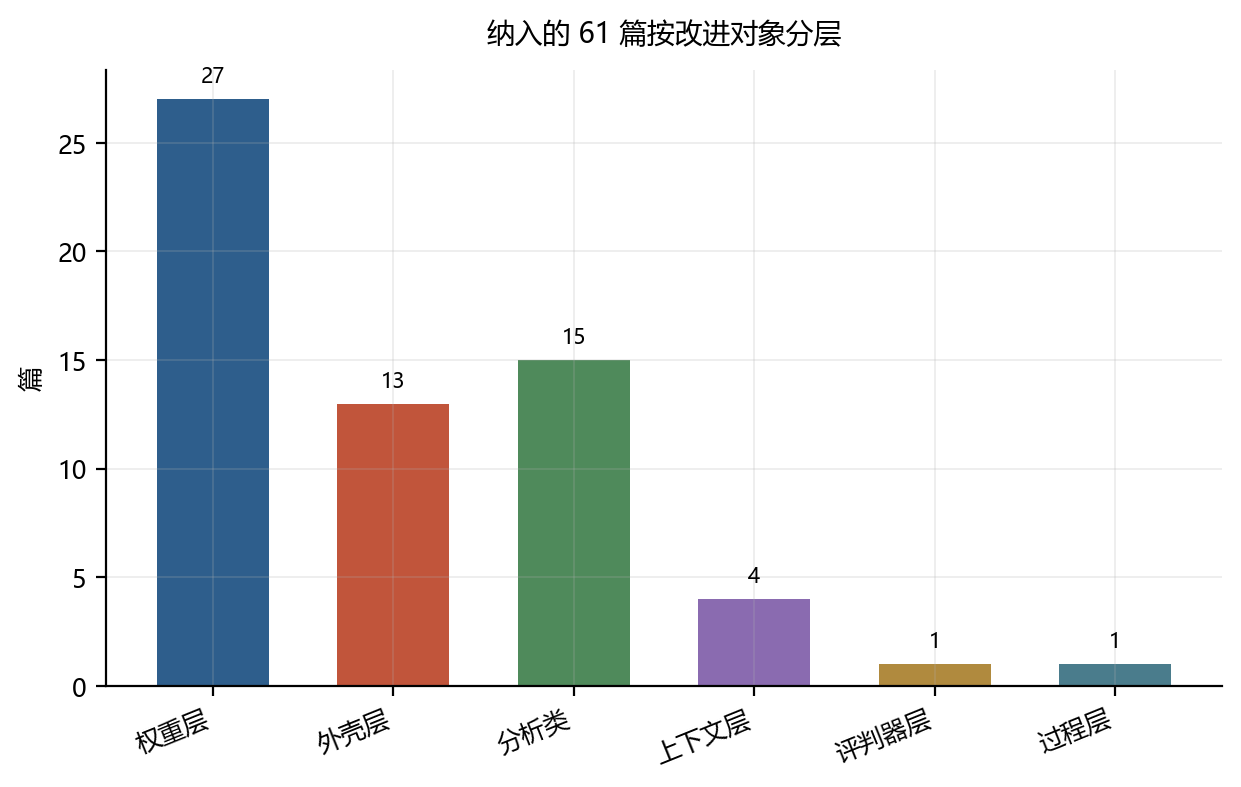
\includegraphics[width=0.86\textwidth]{../figures/fig-2.png}
\caption{图 2　纳入的 61 篇按改进对象分层。权重层占近一半，说明「自我改进」在实际研究里主要指改参数；过程层只有 1 篇，说明最接近 RSI 字面意义的形态才刚出现。}
\label{fig:2}
\end{figure*}

这个分布有一个容易被忽略的含义：\textbf{外壳层 13 篇与上下文层 4 篇加起来 17 篇，比权重层的 27 篇少，但它们的工程采用率远高于权重层。} 原因是成本——改一个提示不需要 GPU 集群。综述界与工业界的注意力分配在这里是错位的。


\section{外部锚点的迁移}

\subsection{一个可统计的趋势}

本文把权重层 27 篇按「奖励从哪来」编码 {\scriptsize\texttt{[c-\hspace{0pt}anchor-\hspace{0pt}migration]}}（图 3）：


\begin{itemize}
  \item \textbf{可判定答案}（answer）20 篇：答案、单元测试、执行器、环境反馈。
  \item \textbf{模型判断}（judge）5 篇：自评，或学到的评判器。
  \item \textbf{统计量替代}（proxy）3 篇：置信度、熵、末 token 概率。
\end{itemize}

\begin{figure*}[t]
\centering
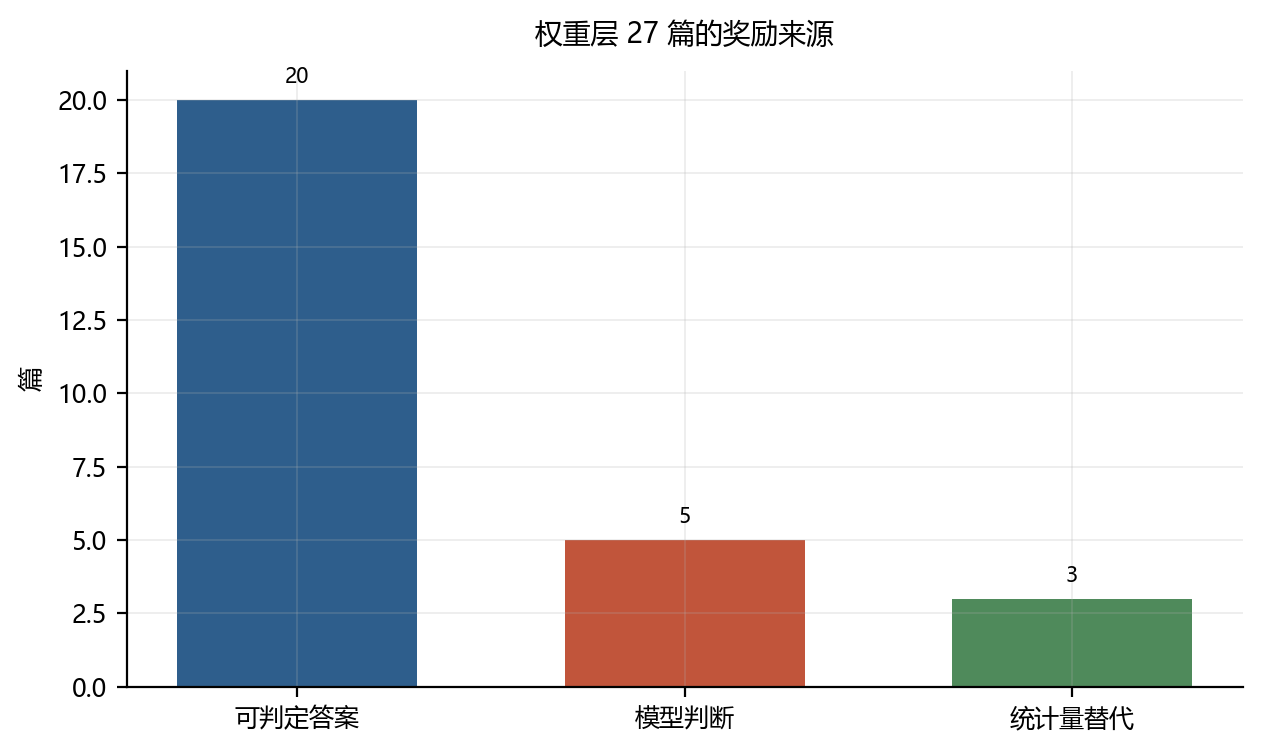
\includegraphics[width=0.86\textwidth]{../figures/fig-3.png}
\caption{图 3　权重层 27 篇的奖励来源。可判定答案仍是主流（20 篇）；模型判断 5 篇、统计量 3 篇，两者都出现在「答案判不了」的开放任务上。}
\label{fig:3}
\end{figure*}

这张图最容易被误读成「大家都不再用答案了」。事实相反：\textbf{四分之三的权重层工作仍在用可判定答案。} 正确的说法是——当答案不可判定时，替代品按「judge \sym{→}{} proxy」的顺序出现，而且这个替代是有代价的。


\subsection{第一段：人写答案}

STaR 的循环写得极清楚：生成推理；答错的题用正确答案回填提示重试；只保留最终答对的推理去微调；重复 {\scriptsize\texttt{[c-\hspace{0pt}star-\hspace{0pt}loop]}}。它的量级声明是与 30 倍大的模型微调可比 {\scriptsize\texttt{[c-\hspace{0pt}star-\hspace{0pt}scale]}}——注意可比对象是 CommensenseQA 上的微调基线，不是通用能力。


ReST 把同样的循环组织成离线批次 {\scriptsize\texttt{[c-\hspace{0pt}rest-\hspace{0pt}offline]}}。SPIN 引入自博弈，但判别基准仍是「人写的回答」{\scriptsize\texttt{[c-\hspace{0pt}spin-\hspace{0pt}anchor]}}：人不再写推理，但仍在定义什么算好。Quiet-STaR 把锚点从标准答案换成后续文本 {\scriptsize\texttt{[c-\hspace{0pt}quiet-\hspace{0pt}star-\hspace{0pt}anchor]}}，锚点开始由语料自带。


这一段里量级最干净的一条来自 Iterative RPO：在 GSM8K 上把准确率从 55.6\% 提到 81.6\% {\scriptsize\texttt{[c-\hspace{0pt}iterative-\hspace{0pt}preference]}}。注意它是同分布评测，不含迁移。


V-STaR 在这一段里提出了一个后来变得很重要的观察：被丢弃的错误解本身是信号 {\scriptsize\texttt{[c-\hspace{0pt}vstar-\hspace{0pt}waste]}}。这句话是后面拒绝采样与过程奖励的前提。


\subsection{第二段：模型当裁判}

2024 年起改进对象上移到评判器：模型用 LLM-as-a-Judge 给自己发奖励，不再依赖独立的奖励模型 {\scriptsize\texttt{[c-\hspace{0pt}evaluator-\hspace{0pt}internalized]}}。Self-Rewarding 报告两条轴同时上升——指令跟随能力，以及给自己发高质量奖励的能力 {\scriptsize\texttt{[c-\hspace{0pt}self-\hspace{0pt}reward-\hspace{0pt}double-\hspace{0pt}axis]}}。


双轴主张是整个内化路线的前提。若评判能力不涨，第二条轴会先饱和——而 Meta-Rewarding 报告的正是这件事：只改答案不改判断会在迭代中迅速饱和；加上「评判自己的判断」后，Llama-3-8B-Instruct 在 AlpacaEval 2 上的胜率从 22.9\% 升到 39.4\% {\scriptsize\texttt{[c-\hspace{0pt}meta-\hspace{0pt}reward-\hspace{0pt}saturation]}}。这是这条路线第一次自我否定，而且是否定自己上一代。


评判器自身也可以被完全自举：Self-Taught Evaluators 不用任何偏好标注，把 Llama3-70B-Instruct 在 RewardBench 上从 75.4 提到 88.3 {\scriptsize\texttt{[c-\hspace{0pt}evaluator-\hspace{0pt}self-\hspace{0pt}taught]}}。


\subsection{第三段：连题都不用出}

2025 年起出现零外部数据自举：模型自己出题、自己解题，课程由「任务接近当前能力边界」这一条件生成，而不是由人编写题库 {\scriptsize\texttt{[c-\hspace{0pt}zero-\hspace{0pt}data]}}。动机写得直白——人类出的题，对未来超越人类的系统学习价值有限 {\scriptsize\texttt{[c-\hspace{0pt}zero-\hspace{0pt}data-\hspace{0pt}incentive]}}。


SSR 走得更远：连自然语言的问题描述都去掉，用测试补丁形式化任务，在两个 SWE 基准上自改进 10.4 与 7.8 个点 {\scriptsize\texttt{[c-\hspace{0pt}ssr-\hspace{0pt}task-\hspace{0pt}formalization]}}。


这一波里最直接把「改自己」当作动作的是 SEAL：模型生成自编辑（改写数据、指定超参、调用工具），再用更新后模型的下游表现作为奖励 {\scriptsize\texttt{[c-\hspace{0pt}seal-\hspace{0pt}weight-\hspace{0pt}edit]}}。它把权重更新本身放进了策略的动作空间，代价是每一次动作都要真跑一次微调才能知道好坏——这是五层里最贵的一次评估。


出题机制也有三条互不相同的路子：与工具交互后出题并自带验证函数（Self-Challenging）、好奇心驱动的自提问（AgentEvolver）、只保留成功轨迹的经验库（SiriuS），而难度接近能力边界时学习效用最高（HS-STaR）{\scriptsize\texttt{[c-\hspace{0pt}task-\hspace{0pt}generation-\hspace{0pt}mechanisms]}}。


还有一条非完全的自举：递归把难题分解成更简单的变体，LADDER 用这一招在本科水平题目上把 Llama 3.2 3B 的准确率从 1\% 提到 82\% {\scriptsize\texttt{[c-\hspace{0pt}recursive-\hspace{0pt}decomposition]}}。起点只有 1\%，\textbf{本文推断}这个量级的相当一部分来自任务被改写而非模型变强——但摘要没有给出对应的对照，故这只是一个待验证的解释，不是结论。


更温和的一条是「用更好的自己当老师」：On-Policy Self-Training 的监督来自特权推理示范，即模型自己更会做的那一版，而不是外部教师 {\scriptsize\texttt{[c-\hspace{0pt}privileged-\hspace{0pt}distill]}}。这与 SEAL 同型，区别只在蒸馏还是改权重。


这里有一个必须说清的区分：\textbf{零数据不等于零监督。} 锚还在，只是从「人出的题」换成了「环境反馈」——测试能不能通过。所以这一段真正做的是把监督外包给环境，而不是取消监督。这个区分在讨论「RSI 能否脱离人类」时是关键：环境是人造的。


\subsection{第四段：用统计量代替判断}

LaSeR 的结论最强：一个解的推理奖励等于它末 token 的自奖励分数，即对某个指定 token 的对数概率差 {\scriptsize\texttt{[c-\hspace{0pt}laser-\hspace{0pt}proxy]}}。这是锚点内移的极限形态——不再问「这个解好不好」，只问「这个模型对这个解有多确信」。


Auxiliary Rewards 用熵的全局变化与局部平滑度替代答案级奖励，在不改 TTRL 的前提下把在线宏平均提高 2.08 个百分点 {\scriptsize\texttt{[c-\hspace{0pt}aux-\hspace{0pt}reward]}}。


还有一种做法是往回走半步：RLSVR 不取消验证，而是把开放任务改造成可自验证的代理环境，用环境内部规则自动产生奖励 {\scriptsize\texttt{[c-\hspace{0pt}rlsvr]}}。这与「零数据」不矛盾——锚点从人写的题换成了人造环境，而环境仍由人设计。


代价必须写清楚：\textbf{统计量与「好」之间的关系是经验性的，不是定义性的。} 答案对错是定义，置信度高低是相关。越往后搬，奖励越容易与目标脱钩，而检测脱钩的手段恰恰是最薄的一环。


四个阶段与它们各自的锚见表 2。


\begin{table*}[t]
\centering
\footnotesize
\setlength{\tabcolsep}{4pt}
\caption{四个阶段与它们各自的锚。阶段划分按「奖励从哪来」，不按时间硬切。}
\label{tab:2}
\begin{tabularx}{\textwidth}{lrlX}
\toprule
阶段 & 时间 & 奖励从哪来 & 代表工作 \\
\midrule
人写答案 & 2022-2024 & 标准答案与人工偏好 & STaR / ReST / SPIN / V-STaR \\
模型当裁判 & 2024-2025 & LLM-as-a-Judge 自评 & Meta-Rewarding / Self-Taught Evaluators \\
零数据自举 & 2025-2026 & 环境反馈（测试能否通过） & Absolute Zero / R-Zero / SSR \\
统计量替代 & 2025-2026 & 置信度与熵 & LaSeR / Auxiliary Rewards \\
\bottomrule
\end{tabularx}
\end{table*}

\section{冻结模型那一支}

\subsection{不是同一件事}

外壳层的工作在机制上与权重层完全不同——它们是「冻结模型、只改外围代码」这一整类，共同点是不需要任何梯度 {\scriptsize\texttt{[c-\hspace{0pt}harness-\hspace{0pt}class]}}：ADAS 用元 agent 写代码发现新 agent，AlphaEvolve 用一个或多个评估器给每次改写背书，而 DGM 的自指性在于它改的是「自己改代码的能力」——代码变更提升的是后续变更的成功率，而不只是任务分数 {\scriptsize\texttt{[c-\hspace{0pt}dgm-\hspace{0pt}self-\hspace{0pt}reference]}}。


SICA 是这一支最干净的展示：不带任何梯度，一个带基本编码工具的 agent 自主编辑自身代码，在 SWE-bench Verified 的随机子集上把成绩从 17\% 提到 53\% {\scriptsize\texttt{[c-\hspace{0pt}sica-\hspace{0pt}no-\hspace{0pt}gradient]}}。这是单 benchmark 子集的小样本结果，数值只应读作「量级」。


这类工作常与权重路线混为一谈，因为两者都自称 self-improving。但把它们混在一起会掩盖最关键的区别：\textbf{外壳可以回滚，权重不能。}


\subsection{代价是样本效率}

ShinkaEvolve 指出这类方法的公认瓶颈：既有代码演化方法需要上千个样本才能找到一个有效解 {\scriptsize\texttt{[c-\hspace{0pt}shinka-\hspace{0pt}efficiency]}}。换言之，外壳路线的「不需要梯度」是用「需要很多次昂贵评估」换来的。


这笔账在论文里常被略过，因为评估成本由检索与执行承担，不显示在训练曲线上。


\subsection{上下文层：被讨论忽略的那一层}

Reflexion 明确不走权重路线，只用语言反馈；Voyager 把经验固化成可执行代码的技能库；AWM 把复用的工作流抽成记忆，在 Mind2Web 与 WebArena 上相对成功率提升 24.6\% 与 51.1\% {\scriptsize\texttt{[c-\hspace{0pt}context-\hspace{0pt}layer]}}。


这一层常被排除在 RSI 之外，理由是它不产生持久的能力改变。但它恰恰是工业界实际在用的那一层，增益量级也不小。把它排除会让「RSI 离落地还有多远」这个问题的答案偏悲观——因为它已经在落地了，只是不叫这个名字。


\section{失效模式}

\subsection{信号侧：判断者与被判断者同源}

模型会系统性高估「高置信度的错误」，形成自我确认循环 {\scriptsize\texttt{[c-\hspace{0pt}self-\hspace{0pt}confirming-\hspace{0pt}loop]}}。原文把它量化成三个量：奖励噪声、策略-奖励耦合、过度/不足奖励偏斜。


这不是调参问题。奖励由模型给出，而模型对错误的置信度与对正确的置信度同源，所以偏差随耦合强度放大。判据饱和是同一个洞的另一种表现：一个是偏置，一个是天花板。


六类失效与它们所在的层见表 3。


\begin{table*}[t]
\centering
\footnotesize
\setlength{\tabcolsep}{4pt}
\caption{六类失效与它们所在的层。「是否结构」一列区分「调参能修」与「改了结构才会变」。}
\label{tab:3}
\begin{tabular}{llll}
\toprule
失效 & 出现在哪一层 & 表现 & 是否结构 \\
\midrule
自我确认循环 & 评判器 / 权重 & 高置信度的错误被系统性高估 & 是（判断者与被判断者同源） \\
判据饱和 & 评判器 / 权重 & 只改答案不改判断时迅速饱和 & 是（同上） \\
Echo Trap & 权重 & 奖励方差悬崖与梯度尖峰 & 未定 \\
熵耗尽 & 权重 & pass@1 上升而策略熵下降 & 是（可验证奖励的固有交换） \\
模型坍缩 & 权重 & 分布尾部不可逆损失 & 是（替换真实数据时） \\
验收门失明 & 外壳 & 重叠防护被逐个删掉而无观测伤害 & 是（门只看得见分数） \\
无停机判据 & 外壳 / 过程 & 停止与模型身份相关而非任务 & 是（缺任务侧终点） \\
\bottomrule
\end{tabular}
\end{table*}

\subsection{训练侧：熵与振荡}

标准 RLVR 提升 pass@1 的代价是策略熵下降 {\scriptsize\texttt{[c-\hspace{0pt}entropy-\hspace{0pt}tradeoff]}}。多轮 agent 强化学习还会出现 Echo Trap：奖励方差出现悬崖、梯度出现尖峰 {\scriptsize\texttt{[c-\hspace{0pt}echo-\hspace{0pt}trap]}}。


还有一层更隐蔽的噪声：一条回答的奖励表示依赖它被随机分到的那一组上下文，因此单次分组实现会给出不可靠的优势估计 {\scriptsize\texttt{[c-\hspace{0pt}gmae-\hspace{0pt}context]}}。在组相对的方法里，这意味着同一个回答在不同 batch 里可能得到不同的优势——它不是数据问题，是估计量问题。


熵这条证据决定了报告口径：只报 pass@1 的方法，无法区分「能力提升」与「多样性被榨干」——两者在 pass@1 上的表现完全一样。


\subsection{分布侧：坍缩及其边界条件}

在自己的输出上训练会造成不可逆的尾部损失（模型坍缩）{\scriptsize\texttt{[c-\hspace{0pt}collapse]}}。规避条件是把各代合成数据与原始真实数据\textbf{累积}而非替换 {\scriptsize\texttt{[c-\hspace{0pt}collapse-\hspace{0pt}avoidable]}}。


但累积不是万能的：采样温度低于 1 时，累积也止不住谱隙收窄。两条证据方向相反却并存，这恰恰是这一节最该保留的形状——\textbf{「坍缩可避免」是一个有条件的结论，条件写在第二篇里。}


\subsection{目标侧：验收门看不见自己在拆防护}

这是本文读到的最不寻常的一条。当多个防护重叠时，删掉其中一个不会产生可观测伤害（被其他防护掩盖），于是验收门只按任务成功率决策，冗余在无人察觉中流失 {\scriptsize\texttt{[c-\hspace{0pt}masked-\hspace{0pt}erosion]}}。


这条失效的特殊性在于：它不是「奖励被 hack」，而是「验收门本身失去了分辨力」。而且它只出现在外壳/代码自改写这一类——因为只有这一类的动作空间里包含「修改防护」。所有基于「用分数当门」的自改进系统都有这个风险，而分数是最常用的门。


\subsection{停止条件}

自我修改何时停止与模型身份强相关，而与任务无关：同一套流程下，有的模型 100\% 声明收敛，有的跑到 101 轮 {\scriptsize\texttt{[c-\hspace{0pt}stop-\hspace{0pt}identity]}}。


这说明「停止」目前不是任务侧的性质，而是模型侧的性质。对无人值守的闭环来说这是一个未解决的工程问题：没有一个与任务挂钩的停机判据。


\section{证据强度}

\subsection{最硬的一条反证}

在 pass@k 取大 k 时，基座模型的分数反而高于 RLVR 训练后的模型，且现有训练没有引出新的推理模式 {\scriptsize\texttt{[c-\hspace{0pt}no-\hspace{0pt}new-\hspace{0pt}capability]}}。


这条证据的分量在于方法：跨多个模型家族、多个 RL 算法、数学/代码/视觉三类基准，用大 k 的 pass@k 作为能力边界指标。它不是说 RL 没用，而是说 \textbf{RL 把已有能力重新加权，没有扩张边界。} 而「自我改进」这个词承诺的正是扩张。


\subsection{审计给出的比例}

在过去 90 篇自称 RSI 的研究中，只有 22\% 审计了两次以上的完整循环，60\% 在未用于选择的任务上评测，而 90\% 报告了产品侧评测 {\scriptsize\texttt{[c-\hspace{0pt}audit-\hspace{0pt}gap]}}（图 4）。


\begin{figure*}[t]
\centering
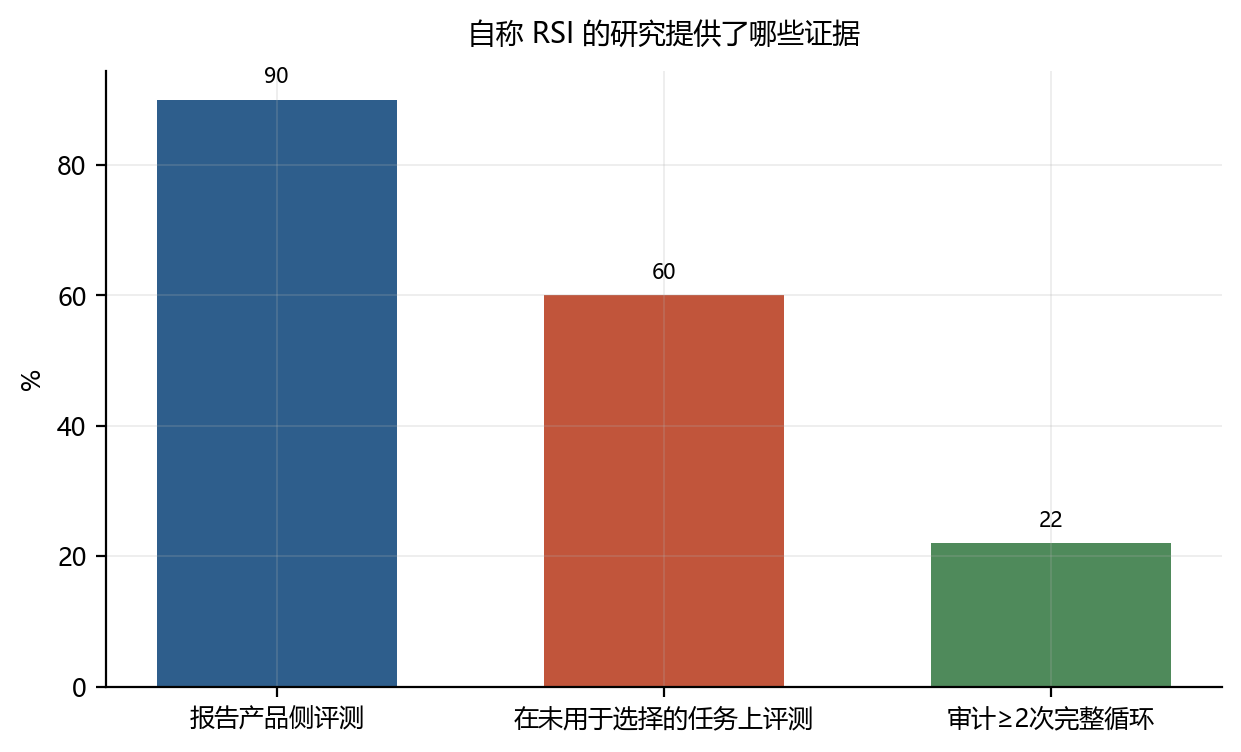
\includegraphics[width=0.86\textwidth]{../figures/fig-4.png}
\caption{图 4　90 篇自称 RSI 的研究中，三类证据的覆盖率。60\% 与 22\% 之间的落差是本文最看重的一个数：在没被选择用过的任务上评测，与把整条循环重跑一遍，是两种完全不同强度的证据。}
\label{fig:4}
\end{figure*}

分母必须说清楚：22\% 的分母是那 90 篇\textbf{自称} RSI 的研究，不是全部 114 篇，更不是所有自改进工作。这个比例的含义是「声明与证据之间的落差有多大」，不是「RSI 不成立」。


\subsection{理论上它应该有效}

自奖励迭代对初始模型的依赖随迭代次数指数衰减，有限样本误差以 O(1/√n) 收敛 {\scriptsize\texttt{[c-\hspace{0pt}theory-\hspace{0pt}decay]}}。


这条与 §7.1 并不矛盾：理论说的是「在模型类与奖励都正确的条件下」，实证说的是「在当前模型与当前奖励下，边界没动」。两者放在一起读，指向同一个位置——\textbf{限制不在迭代次数，在锚的质量。}


\subsection{报告口径的偏差}

61 篇的主指标分布是：准确率 21、成功率 8、pass@1 5、胜率 5、pass@k 2、速度 2，另有 18 篇摘要不报单一主指标 {\scriptsize\texttt{[c-\hspace{0pt}metric-\hspace{0pt}gap]}}（图 5）。


\begin{figure*}[t]
\centering
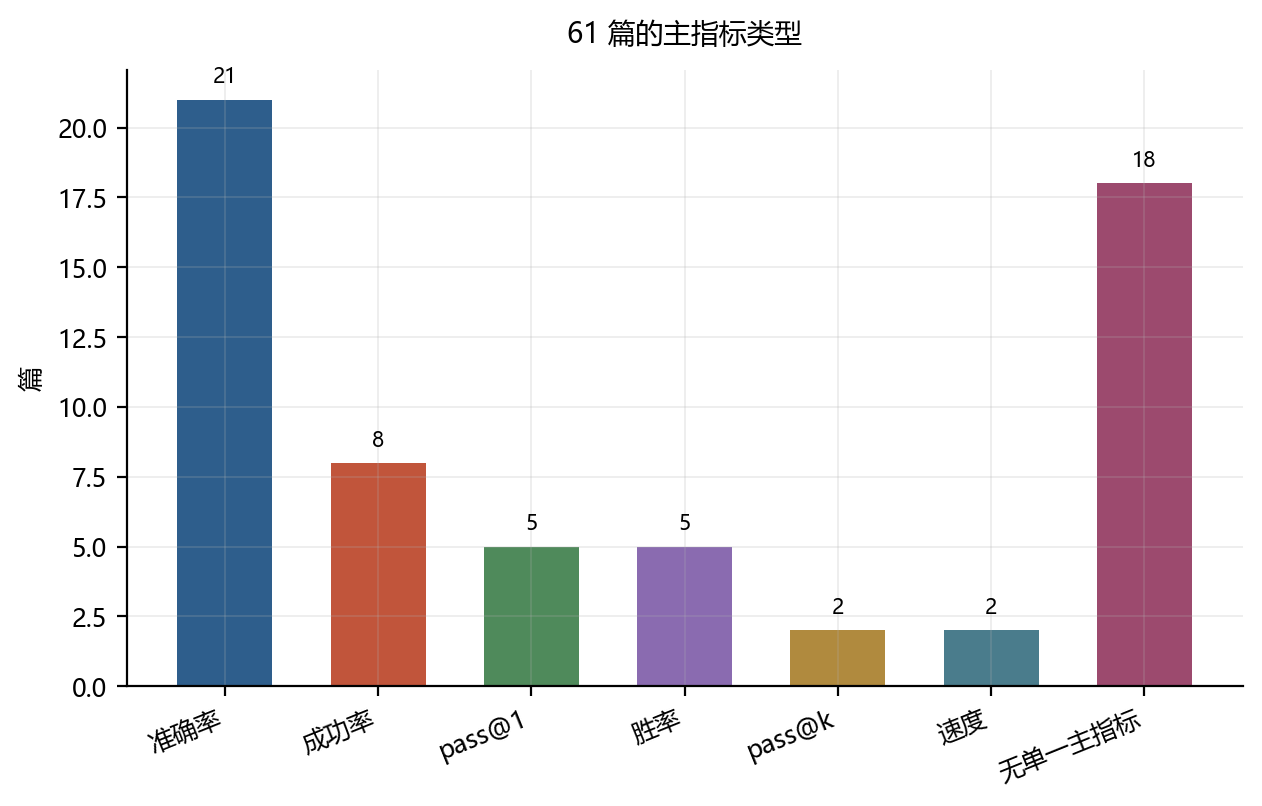
\includegraphics[width=0.86\textwidth]{../figures/fig-5.png}
\caption{图 5　61 篇按摘要中的主指标归类。pass@k 只有 2 篇，而它是唯一能回答「能力边界有没有移动」的指标；速度只有 2 篇，说明成本几乎不在报告范围内。}
\label{fig:5}
\end{figure*}

pass@k 只有 2 篇。这不是巧合：\textbf{被最少报告的指标，正好是最难看的那个。}


\section{过程层：最新的形态}

RSI-Opt 让 meta-agent 依据历史运行证据改写「指导训练优化的策略」，在 5 代演化中让 meta-agent 自己做 CPU 代理实验；Recursa 用并行学习器执行任务、合成局部改进、验证后合并进知识仓库，在留出任务上把全通过率从 30.0\% 提到 55.0\% {\scriptsize\texttt{[c-\hspace{0pt}process-\hspace{0pt}layer]}}。


这一层最接近 RSI 的字面意义：改进的对象包含改进机制本身。它也是最难验证的一层——你无法用一次实验区分「机制变好了」与「这次的任务恰好合适」。


RSI Arena 从另一侧给出可行性证据：十个前沿模型端到端做后训练，各自选数据、实现训练流程、选检查点，十个全部产出了可用助手 {\scriptsize\texttt{[c-\hspace{0pt}rsi-\hspace{0pt}arena]}}。「可用」由 20 个基准与盲评共同判定，不等于达到人类调优水平。


\section{建议}

\subsection{按层决定放开程度}

依据是表 1 的两个性质（可验证性、回滚成本），加上两个可测量的前置条件：验证器强度（与可信参照的一致度）与可恢复性（撤销一次坏改动的代价）{\scriptsize\texttt{[c-\hspace{0pt}verifier-\hspace{0pt}recoverability]}}。


\begin{table*}[t]
\centering
\footnotesize
\setlength{\tabcolsep}{4pt}
\caption{分层放开建议。依据是回滚成本、可验证性，以及验证器强度与可恢复性两个可测前置条件。}
\label{tab:4}
\begin{tabular}{lll}
\toprule
层 & 是否可无人值守 & 理由 \\
\midrule
上下文 & 可以 & 回滚是删记录，验收可直接测任务成功率 \\
外壳 & 有条件 & 回滚便宜，但验收门会掩盖防护流失 \\
评判器 & 需抽检 & 判断者自举引入自我确认偏差，需外部参照集 \\
权重 & 需人工签署 & 回滚成本高、单次更新不可归因，且坍缩不可逆 \\
过程 & 仅限有档案时 & 改进机制被改后，此前验证结论全部失效 \\
\bottomrule
\end{tabular}
\end{table*}

最后一行的理由值得单独说：当被改进的对象包含改进机制本身时，之前所有的验证结论都要作废。这不是保守，是逻辑——你验证的是旧机制。


\subsection{报告建议}

\begin{enumerate}
  \item \textbf{同时报 pass@1 与 pass@k。} 只报前者无法区分能力提升与熵耗尽 {\scriptsize\texttt{[c-\hspace{0pt}entropy-\hspace{0pt}tradeoff]}}。
  \item \textbf{报「未用于选择的任务」上的结果。} 60\% 已经做到，这个数字应该变成 100\% {\scriptsize\texttt{[c-\hspace{0pt}audit-\hspace{0pt}gap]}}。
  \item \textbf{报完整循环的重复次数。} 单次跑通不是 RSI 的证据，22\% 说明这仍是少数派做法。
  \item \textbf{报奖励来源。} judge 与 proxy 的失效模式与 answer 完全不同，混在一起报会掩盖风险 {\scriptsize\texttt{[c-\hspace{0pt}anchor-\hspace{0pt}migration]}}。
\end{enumerate}

\section{效度威胁与局限}

\subsection{全部证据为摘要级}

本档 63 条引文全部是 arXiv 摘要的原文子串，未抓全文。因此凡是「是否做了消融」「表里的具体数值」这类问题，本文一律不下断言。


这是从同类工作的失败里学来的：当证据源比研究对象窄时，缺失会被误读为不存在。摘要是作者用来推销结论的，不是用来汇报实验设计的——用摘要的沉默去论证文献的空白，等于把自己的取材边界写成别人的缺陷。


\subsection{61 篇是编码样本，不是全集}

候选池 1006 篇，人工编码 61 篇。任何百分比都应读作「有这个现象」，不是「比例如此」。


同一件事还有另一个版本，值得写在这里：首轮按记忆列出的 66 个经典 ID 里 11 个是错的，而所有自动校验器都没报错——它们检查引用是否闭合，不检查引用是否指向你以为的那篇论文。\textbf{记忆里的 ID 与文件里的 ID 是两回事，只有逐条核对才能分开。}


\subsection{口径可争议}

分层与奖励来源都是本文的构造。换个口径（例如把 Self-Rewarding 归到评判器层）会得到另一组数。故所有统计都写在 \texttt{corpus\_labels.csv} 里，可由 \texttt{analyze.py} 重算。


\subsection{未覆盖物理 AI}

检索里出现了大量机器人策略的 RSI 工作，它们的证据是物理实验，与文本基准不可直接比较，故排除。这是一个真实的边界：本文的结论对具身场景未必成立。


\section{结论}

四年里，模型确实学会了改进自己——但方式与「RSI」这个词暗示的不同。


\textbf{变的是判断权的位置，不是算法。} 61 篇里没有一篇提出新的优化目标；变化集中在「什么算好」这个判断由谁做出：人写答案、人写测试、模型当裁判、最后用一个标量代替裁判 {\scriptsize\texttt{[c-\hspace{0pt}anchor-\hspace{0pt}migration]}}。每一次内移都换来可扩展性，也都换来一类新的失效 {\scriptsize\texttt{[c-\hspace{0pt}self-\hspace{0pt}confirming-\hspace{0pt}loop]}}{\scriptsize\texttt{[c-\hspace{0pt}masked-\hspace{0pt}erosion]}}。


\textbf{分层比排序更有用。} 与其问「哪个方法更强」，不如问「它在哪一层、失败能不能回滚、改动能不能验证」。这两个性质同向，于是可以直接推出哪一层能放开自动改、哪一层必须人工签署 {\scriptsize\texttt{[c-\hspace{0pt}verifier-\hspace{0pt}recoverability]}}。


\textbf{证据强度是这条路线真正的短板。} 只有 22\% 的自称 RSI 研究审计了两次以上完整循环，唯一能测能力边界是否移动的 pass@k 只有 2/61 篇报告 {\scriptsize\texttt{[c-\hspace{0pt}audit-\hspace{0pt}gap]}}{\scriptsize\texttt{[c-\hspace{0pt}metric-\hspace{0pt}gap]}}。而最强的反证恰恰来自这个指标：大 k 时基座模型反而更高 {\scriptsize\texttt{[c-\hspace{0pt}no-\hspace{0pt}new-\hspace{0pt}capability]}}。


如果要给一句话：\textbf{这个方向已经证明系统可以改进自己，但还没有证明改进的是边界，而不是权重。}


\section{附录 A　可复现性}

\begin{itemize}
  \item 检索：\texttt{fetch\_rsi.py}，16 组 arXiv 检索式取并集，候选池 1006 篇。
  \item 编码：\texttt{codebook.py}，61 篇 × 3 维标签，写入 \texttt{corpus\_labels.csv}。
  \item 证据：\texttt{build\_archive.py} 生成 63 条，\textbf{在写 CSV 之前}逐条校验是否为摘要原文子串，不是就退出、不写文件。
  \item 统计：\texttt{analyze.py} 生成 \texttt{analysis.json}，正文与图表的数字均引自该文件。
  \item 档案校验：\texttt{scripts/validate\_research.py}。
  \item 论文校验：\texttt{scripts/audit\_paper.py}（数值可回溯）、\texttt{scripts/check\_paper.py}（内部自洽）。
\end{itemize}